\chapter{Resultate}

\begin{table}[H]
	\begin{center}
		\caption{Originäre Messergebnisse der Tests}
		\medskip
		\begin{tabulary}{\textwidth}{L C C C C C}
			\toprule
			ID & Ruhe-\acs{HF} in \si{\per\minute} & \acs{HFmax} in \si{\per\minute} & \acs{Wstart} in \si{\watt} & \acs{Wmax} in \si{\watt} & \acs{VO2max} in \si{\litre\per\minute} \\
			\midrule
			\midrule
			1w & 65 & 175 & 40 & 215 & 2,4 \\
			2w & 63 & 183 & 35 & 185 & 2,1 \\
			3w & 53 & 158 & 50 & 225 & 2,7 \\
			4m & 49 & 164 & 50 & 300 & 3,6 \\
			5w & 85 & 187 & 40 & 165 & 2,15 \\
			6w & 65 & 178 & 30 & 205 & 2,55 \\
			7m & 78 & 176 & 55 & 280 & 3,3 \\
			8m & 76 & 195 & 90 & 315 & 4 \\
			9m & 64 & 181 & 40 & 340 & 4,05 \\
			10w & 62 & 168 & 40 & 215 & 2,78 \\
			11m & 90 & 178 & 40 & 215 & 2,6 \\
			12m & 61 & 180 & 75 & 325 & 4 \\
			13m & 62 & 176 & 75 & 275 & 3,45 \\
			14m & 63 & 179 & 100 & 325 & 3,85 \\
			15m & 87 & 193 & 80 & 330 & 4,05 \\
			16w & 84 & 198 & 40 & 240 & 2,98 \\
			17w & 78 & 194 & 50 & 175 & 2 \\
			18w & 68 & 182 & 50 & 225 & 2,7 \\
			19w & 66 & 172 & 40 & 165 & 2,13 \\
			20m & 68 & 197 & 60 & 210 & 2,83 \\
			21m & 92 & 195 & 50 & 275 & 3,4 \\
			22m & 72 & 159 & 50 & 225 & 3,05 \\
			23w & 67 & 173 & 40 & 265 & 3,18 \\
			24m & 94 & 174 & 50 & 250 & 2,83 \\
			25m & 62 & 167 & 50 & 250 & 3,15 \\
			26m & 77 & 169 & 60 & 285 & 3,5 \\
			27m & 86 & 193 & 60 & 285 & 3,58 \\
			28w & 78 & 220 & 40 & 190 & 2,5 \\
			\bottomrule
		\end{tabulary}
		\label{tab:tabelle4}
	\end{center}
\end{table}

Im folgenden Kapitel werden ausgewählte Messergebnisse vorgeführt. Zu Beginn werden einige Plots präsentiert, die für die Auswertung verwendet wurden. Anschließend werden Unterschiede zwischen den Ergebnissen aufgezeigt, die im nächsten Kapitel für die Evaluierung der Methoden diskutiert werden. Alle Messungen wurden ohne Störungen oder Fehler von außerhalb erfolgreich durchgeführt. Die Tabelle \ref{tab:tabelle4} zeigt zu jeder Testperson die vorab ermittelte Ruhe-\acs{HF}, die während der Leistungsdiagnostik \ac{HFmax} sowie die Anfangsbelastung \acs{Wstart}, die Intensität der letzten Belastungsstufe \acs{Wmax} und die \ac{VO2max}. 16 von 28 Personen mussten die Belastungsphase laut eigener Aussage wegen Beinschwäche beenden. Zehn Probanden erreichten nach Selbsteinschätzung ihr konditionales Maximum. Zwei Personen klagten in der letzten Stufe über Atemnot und mussten den Test deshalb abbrechen. Die \acs{HFmax} sowie die \acs{VO2max} werden im nächsten Kapitel in die Diskussion involviert und wurden erhoben, um z.B. den Status der Ausbelastung eines Probanden zu reproduzieren.

\section{Plots für die Schwellenbestimmung}

\subsection{Manuelle Auswertung}

Im Folgenden werden zwei Beispielplots verschiedener Probanden für die manuelle Bestimmung der Schwellen durch die menschlichen Rater gezeigt, beginnend mit Abb. \ref{pic:pic15} für Probandin 6w. Sie bestehen insgesamt aus sechs Grafik-Feldern. Im 1. Feld der oberen Reihe ist der V-Slope in Form eines schwarzen Graphen zu sehen. Das 2. Feld beinhaltet das \acs{EQO2} als blauen und das \acs{EQCO2} als orangefarbenen Graphen. Als hellblauer Graph ist im 3. Feld der \acs{RQ} aufgetragen. Im 4. Feld, an erster Stelle der unteren Reihe, ist der Vergleich von \acs{VE} zu \acs{VCO2} als schwarzer Graph geplottet. Alle Felder, welche zur Schwellenbestimmung genutzt wurden, enthalten zur erleichterten Auswertung den Verlauf der \acs{HF} als rosafarbenen gestrichelten Graphen. Je nach Skalierung der Achsen, kann diese unterschiedliche Formen haben und dient nur zum Vergleich mit den Graphen im selben Plot. Sie wird individuell durch eine zweite (rechte) Y-Achse skaliert. In Feld 5 und 6 werden \acs{VE} sowie \acs{VO2} mit der Leistung (hier als "`Watt"' bezeichnet) in Relation gesetzt. Die Kreuze in den Graphen stellen die Mittelwerte einer Stufe dar und spiegeln in ihrer Menge die Anzahl der gefahrenen Belastungsstufen wider.

\begin{figure}[H]
	\centering
	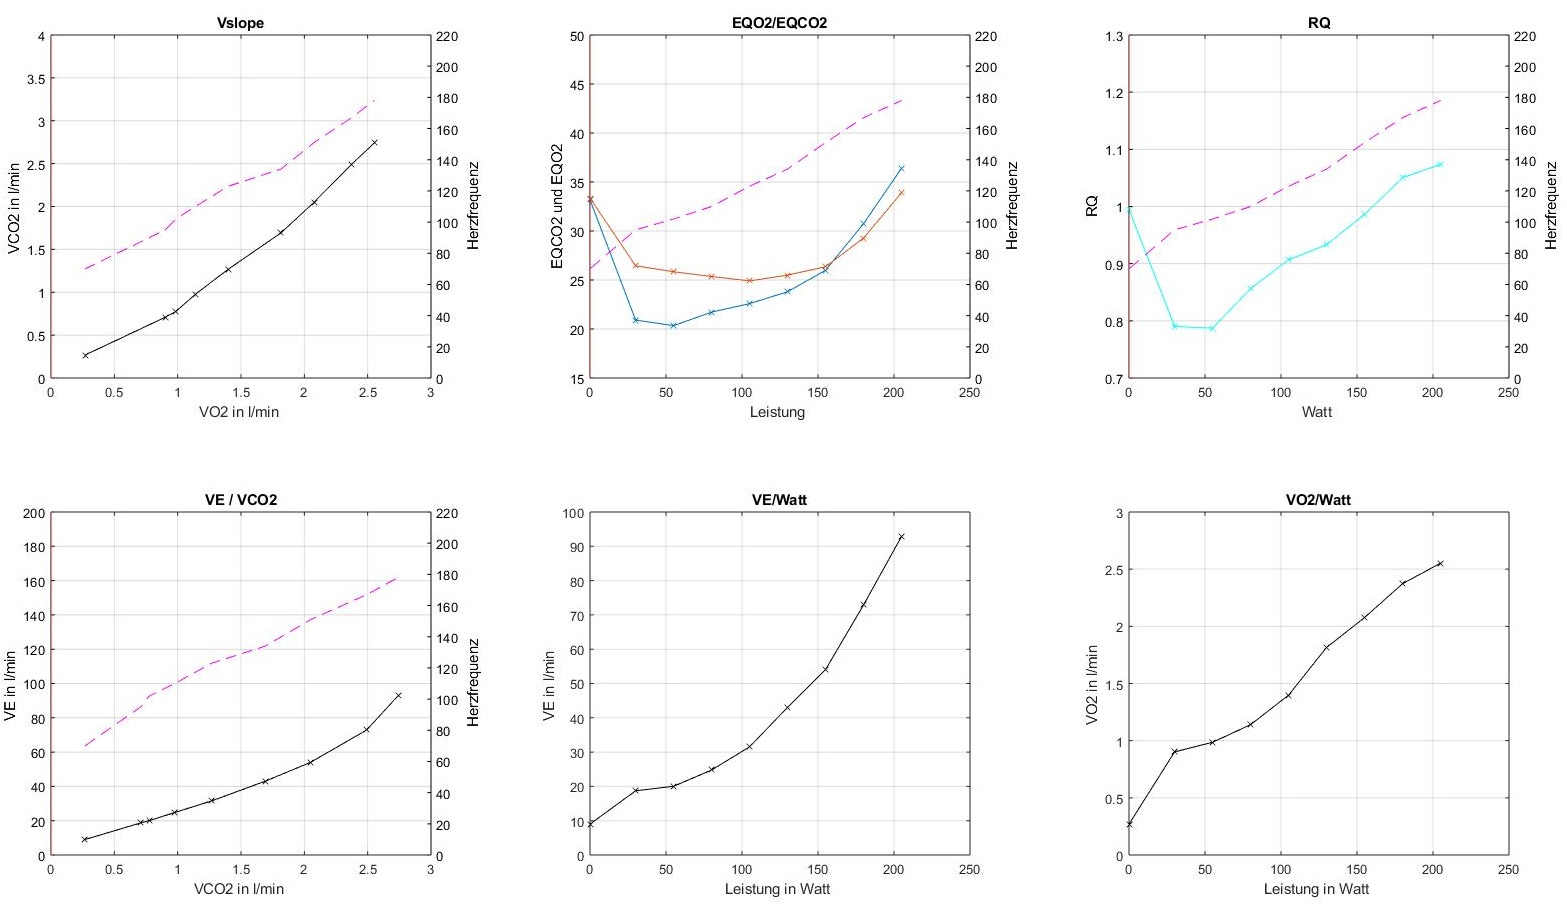
\includegraphics[width=\textwidth]{Bilder/plot_6w.jpg}
	\caption{6-Felder-Grafik von Probandin 6w}
	\label{pic:pic15}
\end{figure}
%
\begin{figure}[H]
	\centering
	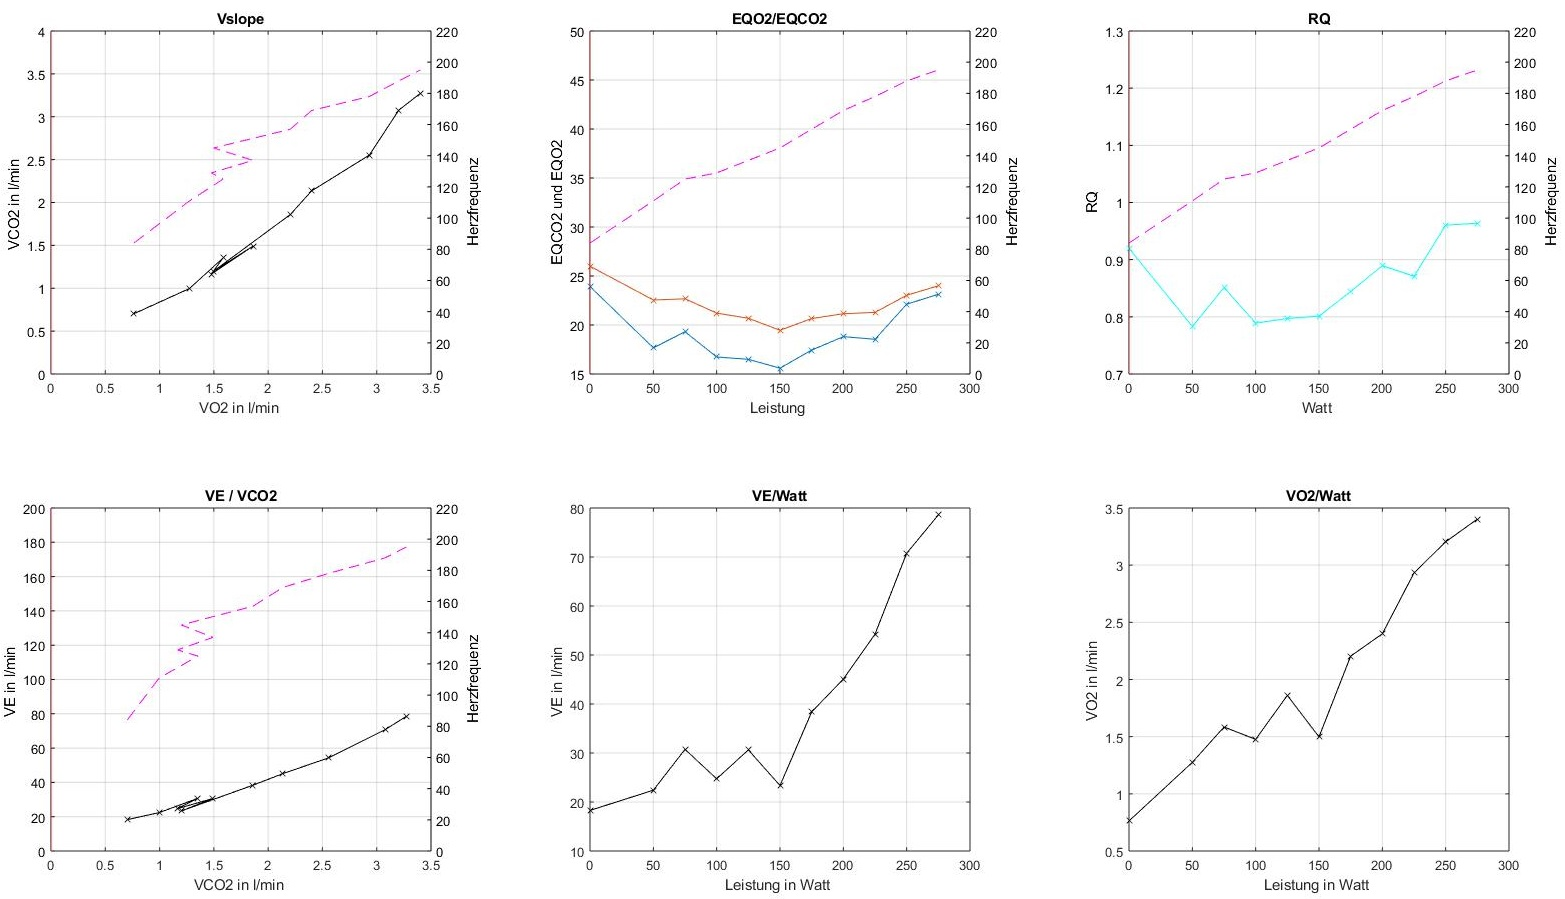
\includegraphics[width=\textwidth]{Bilder/plot_21m.jpg}
	\caption{6-Felder-Grafik von Proband 21m}
	\label{pic:pic16}
\end{figure}

Abb. \ref{pic:pic16} zeigt eine weitere 6-Felder-Grafik von Proband 21m. Er zeigt unregelmäßige Graphen und es ist zu sehen, dass der RQ (hellblau) während des Tests nie den Wert eins erreichte. Außerdem tritt in der \acs{EQCO2}-Kurve kein signifikanter Anstieg zum Ende der Leistungsdiagnostik auf. Die Graphen im 5. und 6. Feld besitzen in Abb. \ref{pic:pic15} stetige Steigungen. In Abb. \ref{pic:pic16} schwanken die Kurven zwischen einzelnen Messpunkten. Die übrigen Plots weisen an den betroffenen Stufen Analogien zu diesen Schwankungen auf. Beispielsweise sinkt in Feld 1 die \acs{VO2} zwischen Messpunkt 3 und 4 im Vergleich zur \acs{VCO2}. Dies ist auch im 6. Feld der Fall. Identisch verhält sich die \acs{VCO2} sowohl in Feld 1, als auch im 4. Feld zusammen mit der \acs{VE}. Eine vergleichbare Schwankung ist im nebenstehenden Feld 5 zu sehen. \acs{VE}/Watt und \acs{VO2}/Watt wurden genutzt, um Messfehler zu detektieren und werden im nachfolgenden Kapitel weiter behandelt.

\subsection{Algorithmische Auswertung}

In diesem Abschnitt werden Plots präsentiert, die zusätzlich eine algorithmische Schwellenbestimmung des MATLAB-Programms enthalten. Hierdurch wurde für jeden Probanden eine zweite Bilddatei erstellt, welche die VT1 und VT2 bereits in Form von vertikalen Linien beinhaltet und durch eine Angabe für die \acs{HF} an der jeweiligen Schwelle ergänzt ist. In Feld 5 dieser Plots wurde im Vergleich mit der \acs{VE} die Leistung durch die \acs{HF} ersetzt und es wurden bereits Trainingsbereiche eingefügt, die ebenfalls durch farbige vertikale Linien gekennzeichnet und in einer Legende mit Wertebereichen beschrieben sind. Es werden \ac{REKOM}, \ac{GA1}, \ac{GA2}, \ac{EW} und Leistung als Trainingszonen definiert. Dieser Plot diente dem Testlauf eines neuen Modells zur Trainingssteuerung. Die Entwicklung und Implementierung dieses Modells basierte auf den Erkenntnissen zur Schwellenbestimmung und wurde nachträglich eingefügt. Im Kapitel Diskussion wird näher darauf eingegangen.
%
\begin{figure}[H]
	\centering
	\noindent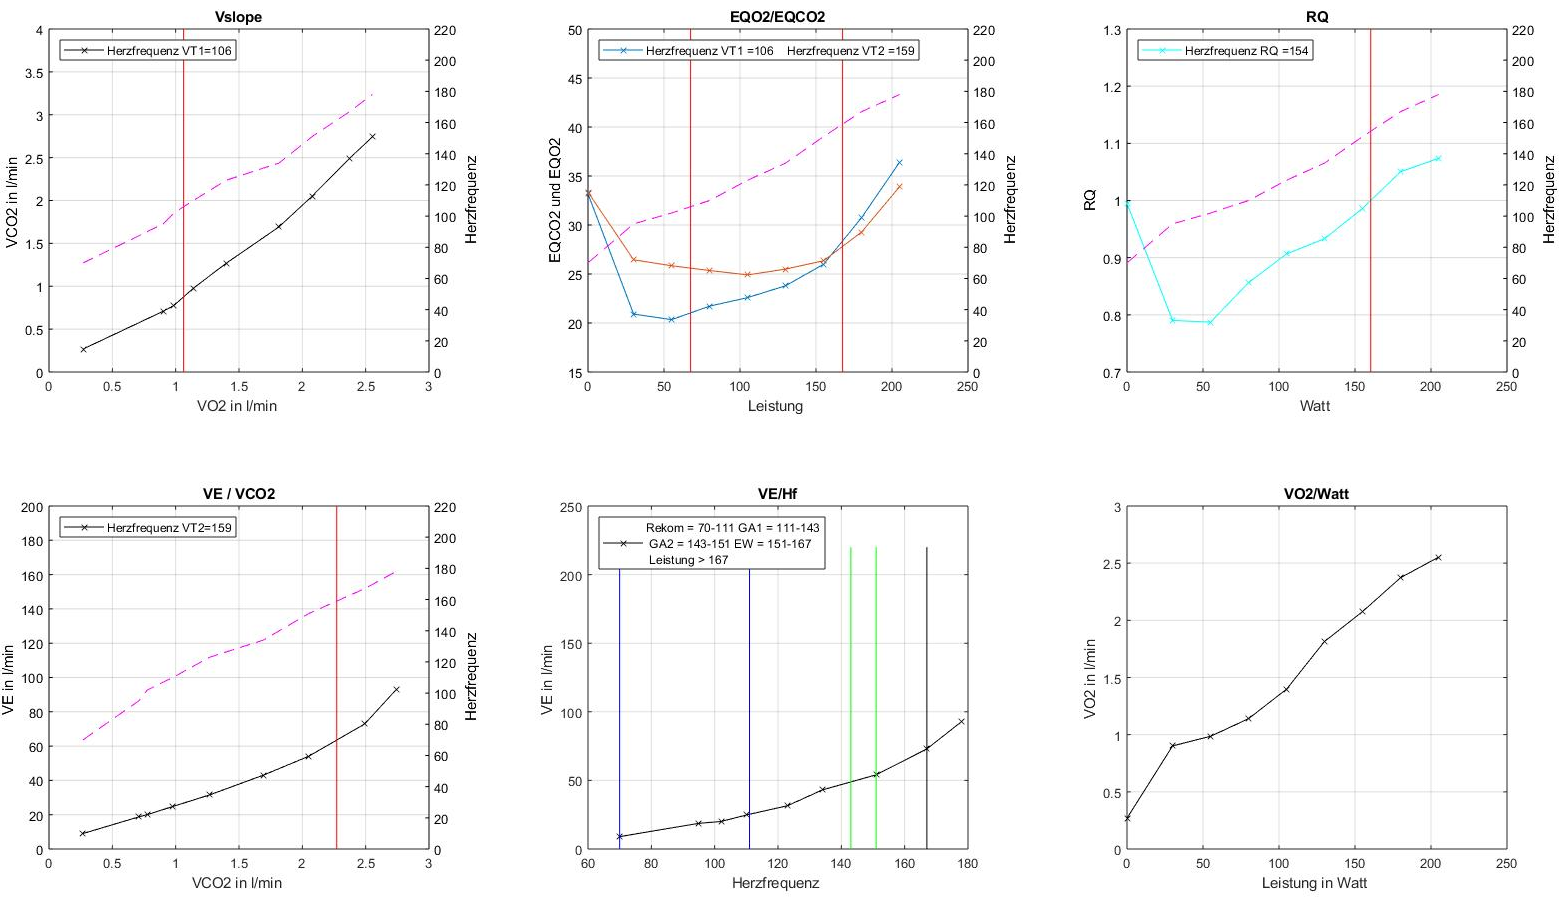
\includegraphics[angle=0,width=\linewidth,keepaspectratio]{Bilder/auto_6}
	\caption[6-Felder-Grafik von Probandin 6w mit algorithmischen Schwellenmarkierungen]{6-Felder-Grafik von Probandin 6w mit algorithmischen Schwellenmarkierungen: \textsl{V-Slope} = \SI{106}{\per\minute}, \textsl{\acs{EQO2}} = \SI{106}{\per\minute}, \textsl{\acs{EQCO2}} = \SI{159}{\per\minute}, \textsl{\acs{VE}/\acs{VCO2}} = \SI{159}{\per\minute}}
	\label{pic:pic17}
\end{figure}
%
\begin{figure}[H]
	\centering
	\noindent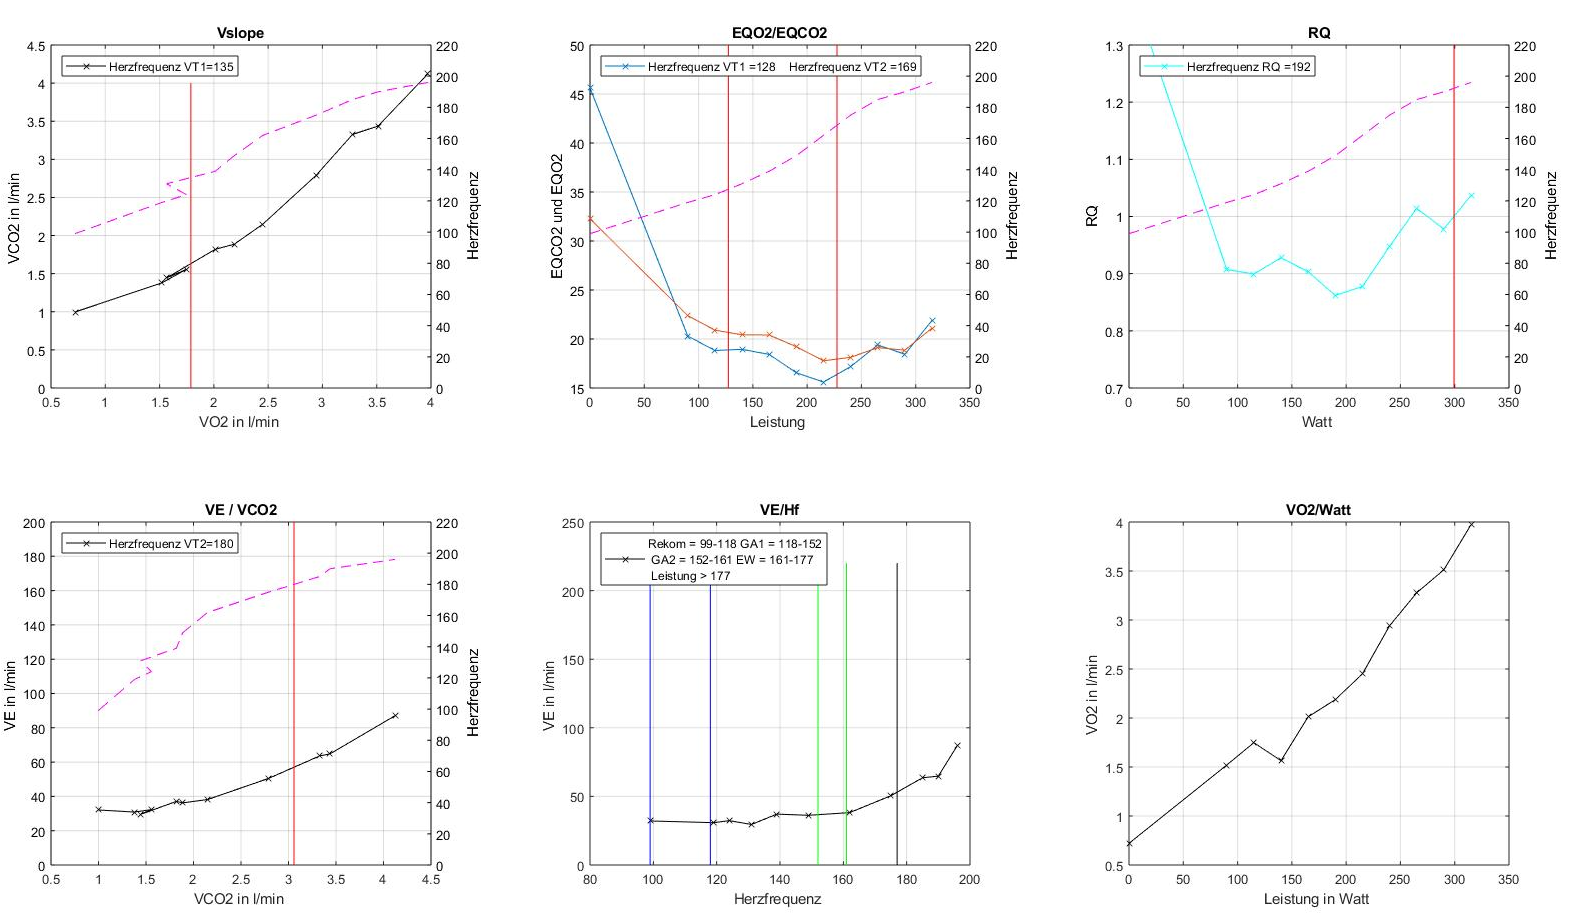
\includegraphics[angle=0,width=\linewidth,keepaspectratio]{Bilder/auto_8}
	\caption[6-Felder-Grafik von Proband 8m mit algorithmischen Schwellenmarkierungen]{6-Felder-Grafik von Proband 8m mit algorithmischen Schwellenmarkierungen: \textsl{V-Slope} = \SI{135}{\per\minute}, \textsl{\acs{EQO2}} = \SI{126}{\per\minute}, \textsl{\acs{EQCO2}} = \SI{169}{\per\minute}, \textsl{\acs{VE}/\acs{VCO2}} = \SI{180}{\per\minute}}
	\label{pic:pic18}
\end{figure}
%
\begin{figure}[H]
	\centering
	\noindent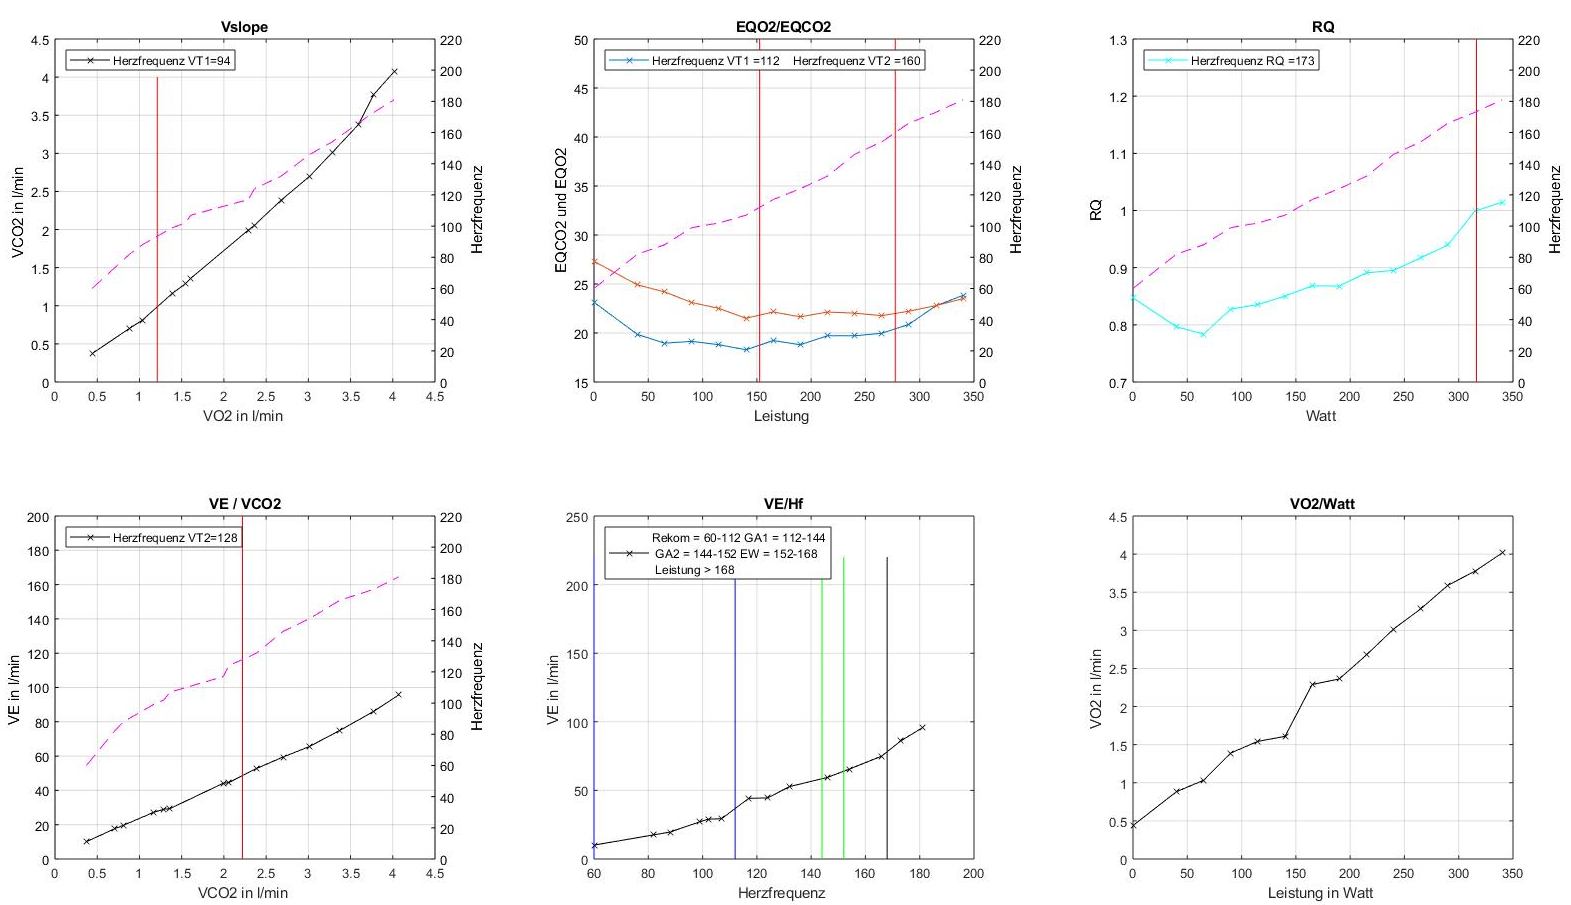
\includegraphics[angle=0,width=\linewidth,keepaspectratio]{Bilder/auto_9}
	\caption[6-Felder-Grafik von Proband 9m mit algorithmischen Schwellenmarkierungen]{6-Felder-Grafik von Proband 9m mit algorithmischen Schwellenmarkierungen: \textsl{V-Slope} = \SI{94}{\per\minute}, \textsl{\acs{EQO2}} = \SI{112}{\per\minute}, \textsl{\acs{EQCO2}} = \SI{160}{\per\minute}, \textsl{\acs{VE}/\acs{VCO2}} = \SI{128}{\per\minute}}
	\label{pic:pic19}
\end{figure}
%
\begin{figure}[H]
	\centering
	\noindent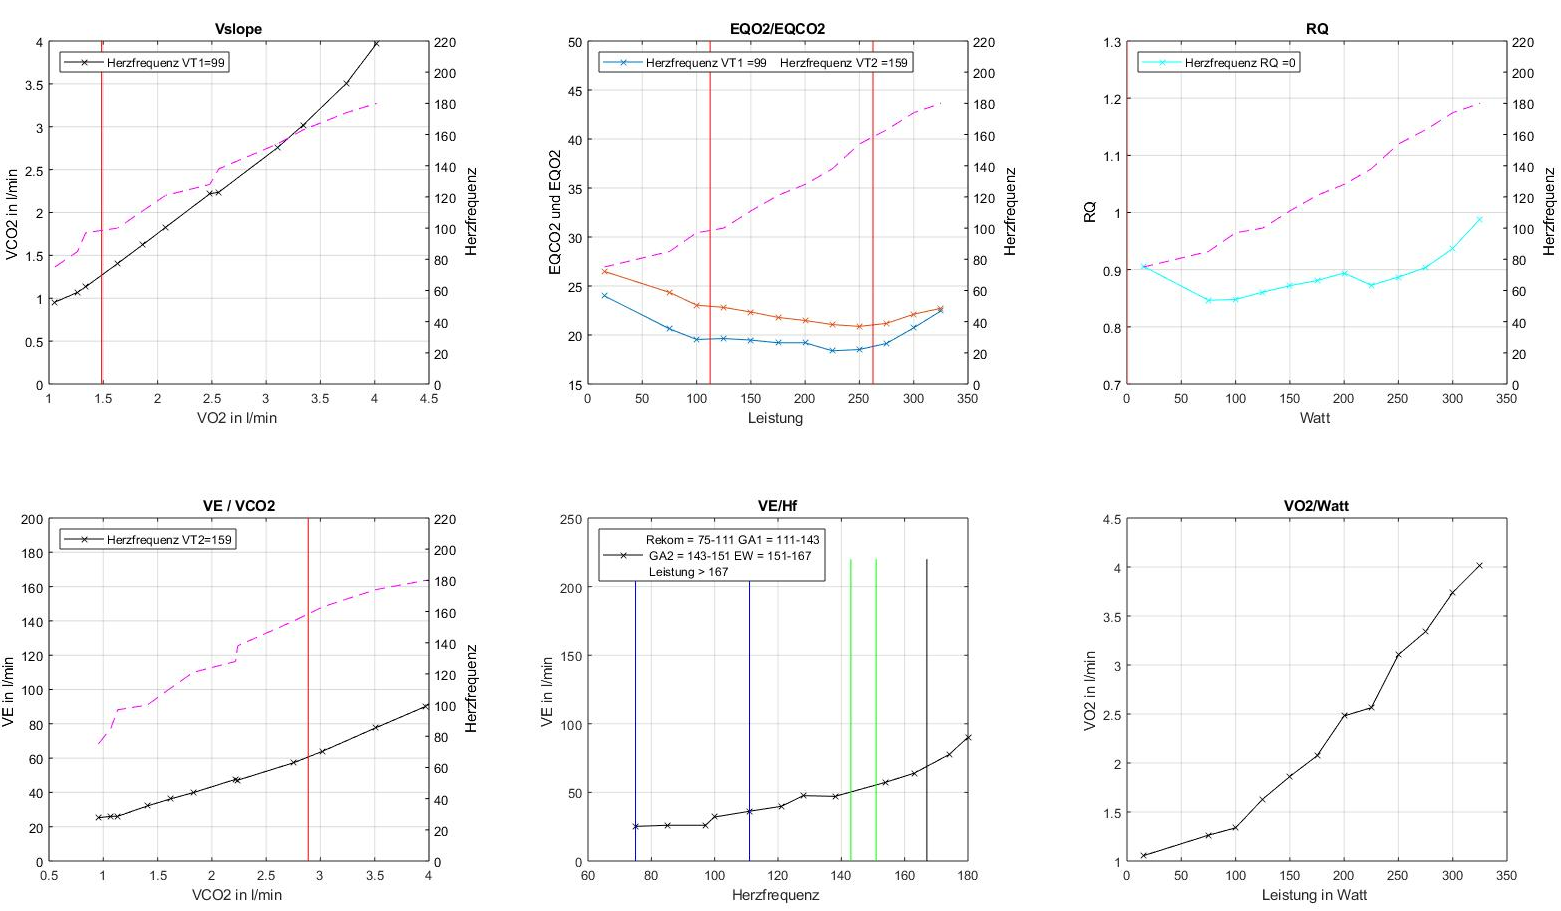
\includegraphics[angle=0,width=\linewidth,keepaspectratio]{Bilder/auto_12}
	\caption[6-Felder-Grafik von Proband 12m mit algorithmischen Schwellenmarkierungen]{6-Felder-Grafik von Proband 12m mit algorithmischen Schwellenmarkierungen: \textsl{V-Slope} = \SI{99}{\per\minute}, \textsl{\acs{EQO2}} = \SI{99}{\per\minute}, \textsl{\acs{EQCO2}} = \SI{159}{\per\minute}, \textsl{\acs{VE}/\acs{VCO2}} = \SI{159}{\per\minute}}
	\label{pic:pic20}
\end{figure}
%
\begin{figure}[H]
	\centering
	\noindent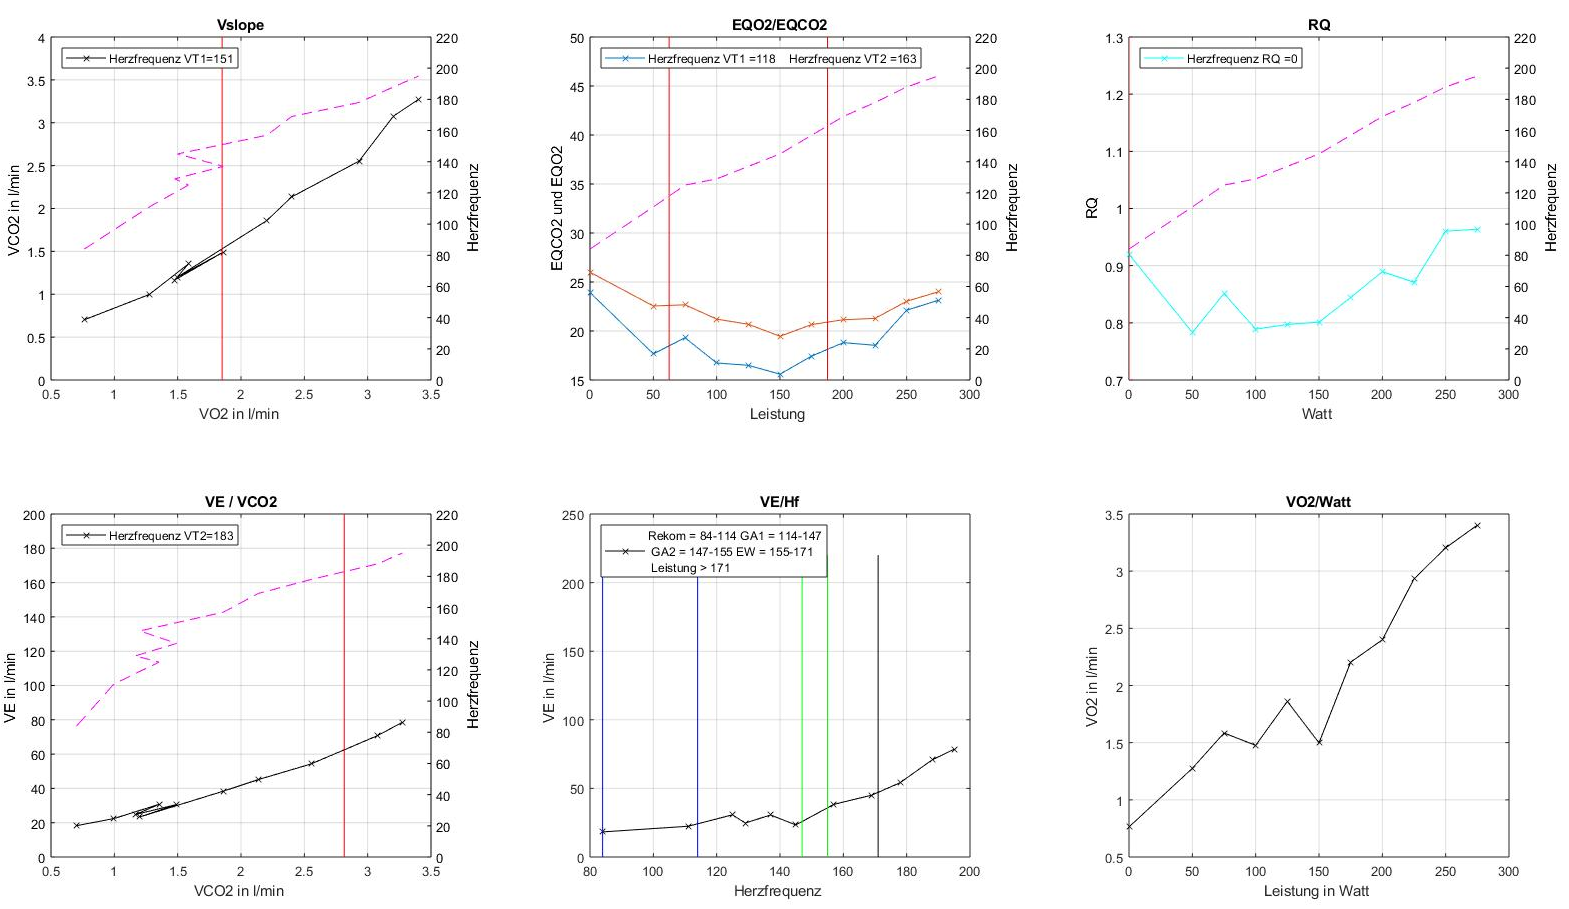
\includegraphics[angle=0,width=\linewidth,keepaspectratio]{Bilder/auto_21}
	\caption[6-Felder-Grafik von Proband 21 mit algorithmischen Schwellenmarkierungen]{6-Felder-Grafik von Proband 21 mit algorithmischen Schwellenmarkierungen: \textsl{V-Slope} = \SI{151}{\per\minute}, \textsl{\acs{EQO2}} = \SI{118}{\per\minute}, \textsl{\acs{EQCO2}} = \SI{163}{\per\minute}, \textsl{\acs{VE}/\acs{VCO2}} = \SI{183}{\per\minute}}
	\label{pic:pic21}
\end{figure}
%
In Abb. \ref{pic:pic17} erfolgte die Schwellenbestimmung für Probandin 6w nach acht Stufen, bei der jeweils beide Methoden für VT1 sowie  VT2 identische Ergebnisse erbrachten. Im blauen \acs{EQO2}-Graphen ist zu sehen, dass VT1 zwischen Tiefpunkt und darauffolgendem Messpunkt bestimmt wurde. Am \acs{EQCO2} ist erkennbar, dass VT2 beim ersten signifikanten Kurvenanstieg markiert wurde. Bei der Probandin stieg in der 7. Stufe der RQ über eins hinaus. Die mithilfe dieser Methode erhobene VT2 liegt bei einer \acs{HF} von \SI{154}{\per\minute}.\\
Der Plot in Abb. \ref{pic:pic18} entstand für Proband 8m. \acs{HF} und V-Slope in Feld 1 sowie \acs{VE}/\acs{VCO2} in Feld 4 sind zwischen Stufe 2 und 4 nicht differenzierbar. Die \acs{VO2} fällt im 6. Feld zwischen diesen Stufen. Der RQ schwankt zwischen den letzten zwei Messungen um den Wert eins herum. Die Software bestimmte den zweiten Anstieg über eins bei \SI{192}{\per\minute} als VT2.\\
Abb. \ref{pic:pic19} stellt den Plot von Proband 9m dar, der sogar 13 Belastungsstufen bewältigte. Mit RQ = 1 wurde in der letzten Stufe bei \SI{173}{\per\minute} VT2 markiert. In Feld 5 und 6 sind Schwankungen im Anstieg von \acs{VE} und \acs{VO2} in Relation zur \acs{HF} bzw. Belastung erkennbar.\\ 
In Abb. \ref{pic:pic20} ist eine Auswertung für Proband 12m zu sehen, welcher wiederum insgesamt elf Stufen fuhr. Hier wurden ebenfalls VT1 und VT2 mit beiden jeweiligen Methoden gleich bestimmt. Der RQ in Feld 3 stieg nicht über eins. Da die VT2 durch diese Methode vom Algorithmus nicht bestimmt werden konnte, ist der Wert null in der Legende angegeben. Im V-Slope sind mehrere Knickpunkte zu erkennen. Im 2. Feld tritt der Tiefpunkt von \acs{EQO2} erst in der 7. Stufe auf. \acs{EQCO2} sinkt an diesem Punkt noch, steigt jedoch ab der nächsten Stufe an. Im \acs{VO2}/Watt-Vergleich ist ein Knickpunkt mit geringerer Steigung ebenfalls nach der 7. Stufe zu sehen.\\
Der fünfte Beispielplot in Abb. \ref{pic:pic21} zeigt die Ergebnisse des Probanden 21m analog zu Abb. \ref{pic:pic16} inklusive der Schwellenbestimmung der Software. Dieser Proband bewältigte zehn Belastungsstufen. Im 6. Feld ist eine schwankende Steigung der \acs{VO2} in Relation zur Belastung zwischen Stufe 2 und 5 erkennbar. Diese Schwankungen tauchen auch im V-Slope und bei \acs{VE}/\acs{VCO2} sowie RQ auf. Auch hier unterscheiden sich die Bestimmungen für VT1 durch V-Slope und \acs{EQO2} sowie jene für VT2 anhand von \acs{EQCO2} oder \acs{VE}/\acs{VCO2}. Wie bereits in Abschnitt 3.3.1 erwähnt, erreichte der RQ dieses Probanden auch nicht den Wert eins.

\section{Ergebnisse der Schwellenbestimmung}

\subsection{Ergebnisse für VT1}

In Tab. \ref{tab:tabelle5} werden die Ergebnisse der VT1-Bestimmung der Rater und der Software für alle 28 Testpersonen verglichen. In sechs Spalten wird, geordnet nach Methode und Rater, die \acs{HF} aufgeführt, die an Stelle der VT1 abgelesen bzw. durch die Software bestimmt wurden. Es werden dabei auch nebeneinander die Methoden in direkte Relation gesetzt. Bei einigen Probanden sind zwischen den jeweiligen Ratern bzw. den beiden Methoden Differenzen zu sehen. Zur Visualisierung der Übereinstimmungen bzw. Unterschiede zwischen den VT1 von Ratern und Software wurde deshalb für jede Methode ein Netzdiagramm erstellt.

\begin{table}[H]
	\begin{center}
		\caption{Ergebnisse für die VT1 in \si{\per\minute}}
		\medskip
		\begin{tabulary}{\textwidth}{L@{\hspace{3em}} C C C C C C}
			\toprule
			& \multicolumn{2}{c}{\textbf{Rater 1}} & \multicolumn{2}{c}{\textbf{Rater 2}} & \multicolumn{2}{c}{\textbf{Software}} \\
			\midrule
			ID & V-Slope & \acs{EQO2} & V-Slope & \acs{EQO2} & V-Slope & \acs{EQO2} \\
			\midrule
			\midrule
			1w & 109 & 133 & 133 & 130 & 101 & 132 \\
			2w & 119 & 120 & 126 & 126 & 121 & 121 \\
			3w & 115 & 116 & 118 & 116 & 97 & 117 \\
			4m & 98 & 99 & 100 & 100 & 98 & 98 \\
			5w & 118 & 120 & 115 & 122 & 124 & 124 \\
			6w & 102 & 106 & 106 & 109 & 106 & 106 \\
			7m & 105 & 115 & 105 & 145 & 105 & 114 \\
			8m & 120 & 126 & 155 & 168 & 135 & 128 \\
			9m & 110 & 115 & 92 & 116 & 94 & 112 \\
			10w & 118 & 117 & 118 & 118 & 117 & 117 \\
			11m & 114 & 115 & 135 & 135 & 114 & 135 \\
			12m & 142 & 140 & 148 & 158 & 99 & 99 \\
			13m & 115 & 116 & 116 & 116 & 116 & 116 \\
			14m & 116 & 118 & 129 & 132 & 134 & 110 \\
			15m & 118 & 118 & 145 & 146 & 146 & 120 \\
			16w & 130 & 150 & 152 & 153 & 130 & 130 \\
			17w & 138 & 138 & 135 & 138 & 136 & 136 \\
			18w & 135 & 137 & 138 & 138 & 102 & 140 \\
			19w & 122 & 122 & 138 & 152 & 135 & 126 \\
			20m & 116 & 116 & 110 & 110 & 114 & 114 \\
			21m & 118 & 115 & 160 & 152 & 151 & 118 \\
			22m & 108 & 108 & 109 & 110 & 110 & 101 \\
			23w & 110 & 120 & 110 & 146 & 111 & 87 \\
			24m & 113 & 115 & 115 & 117 & 117 & 111 \\
			25m & 100 & 100 & 100 & 135 & 104 & 104 \\
			26m & 140 & 140 & 141 & 140 & 112 & 142 \\
			27m & 110 & 130 & 130 & 132 & 134 & 134 \\
			28w & 103 & 120 & 108 & 120 & 109 & 122 \\
			\bottomrule
		\end{tabulary}
		\label{tab:tabelle5}
	\end{center}
\end{table}
%
Abb. \ref{pic:pic22} zeigt die Netzdiagramme für die VT1. Abb. \ref{subpic:pic1} vergleicht dabei die \acs{HF} für VT1, die von Ratern und Software durch den V-Slope bestimmt wurden. In Abb. \ref{subpic:pic2} ist das gleiche für \acs{EQO2} dargestellt. Eine Skala von \SIrange{0}{160}{\per\minute} definiert die \acs{HF}, die an konzentrischen Kreisen abgelesen werden kann. Der äußere Kreis stellt eine zweite Skala dar, welche mit den IDs der Probanden beschriftet ist. Radial sind zu jeder ID die Messwerte in den Diagrammen eingesetzt. Zusammen bilden die Messpunkte ein farbig schraffiertes Netz. Die schwarze Schraffur visualisiert das Netz des 1. Raters, die rote das des 2. Raters. Die grüne Schraffur verkörpert die VT1-Werte der Software. Unterschiedliche Kontraste markieren Bereiche, in denen sich die individuellen Schwellenbestimmungen überlappen.

\begin{figure}[H]
	\centering
	\begin{subfigure}[c]{0.45\textwidth}
		\centering
		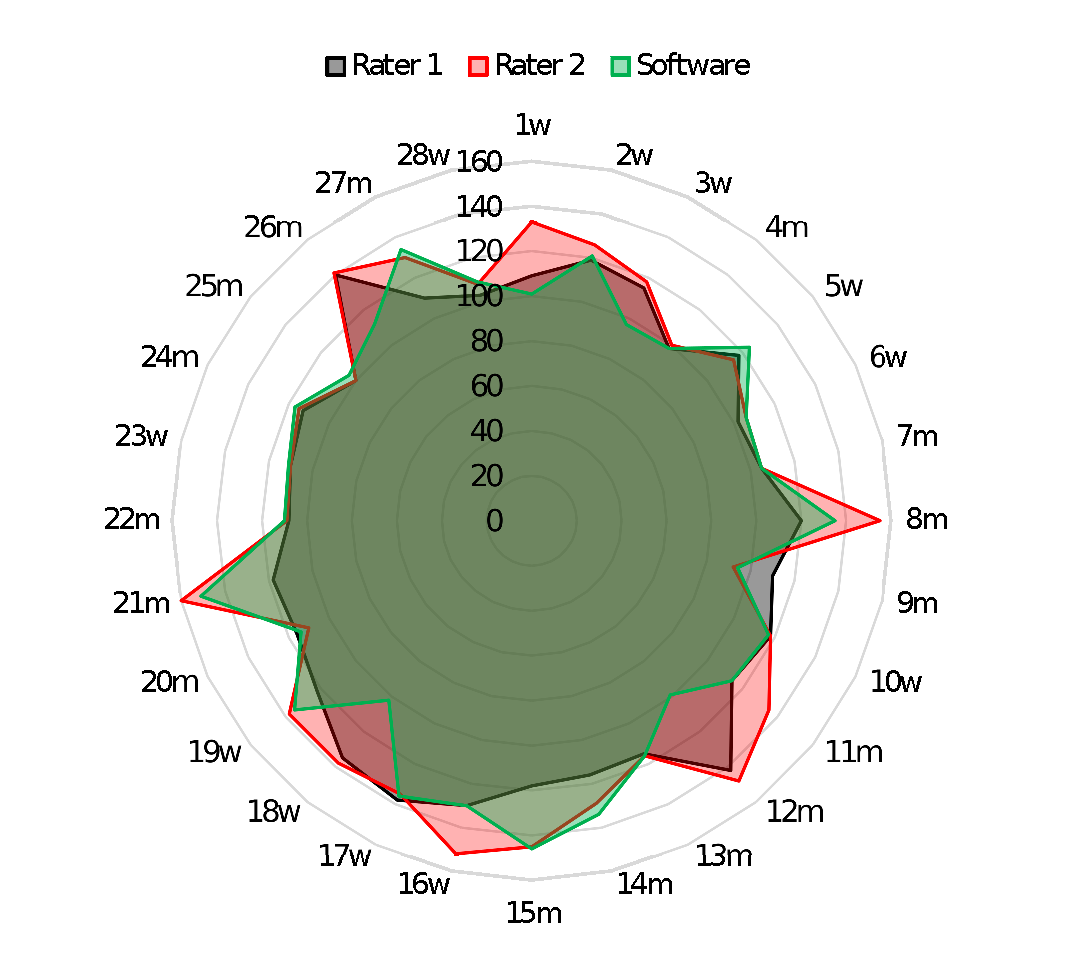
\includegraphics[scale=0.73]{Bilder/v-slope_net}
			\subcaption[Vergleich der VT1-Bestimmungen durch V-Slope]{Vergleich der VT1-Bestimmungen durch V-Slope zwischen Ratern und Software}
			\label{subpic:pic1}
	\end{subfigure}%
	\hfil
	\begin{subfigure}[c]{0.45\textwidth}
		\centering
		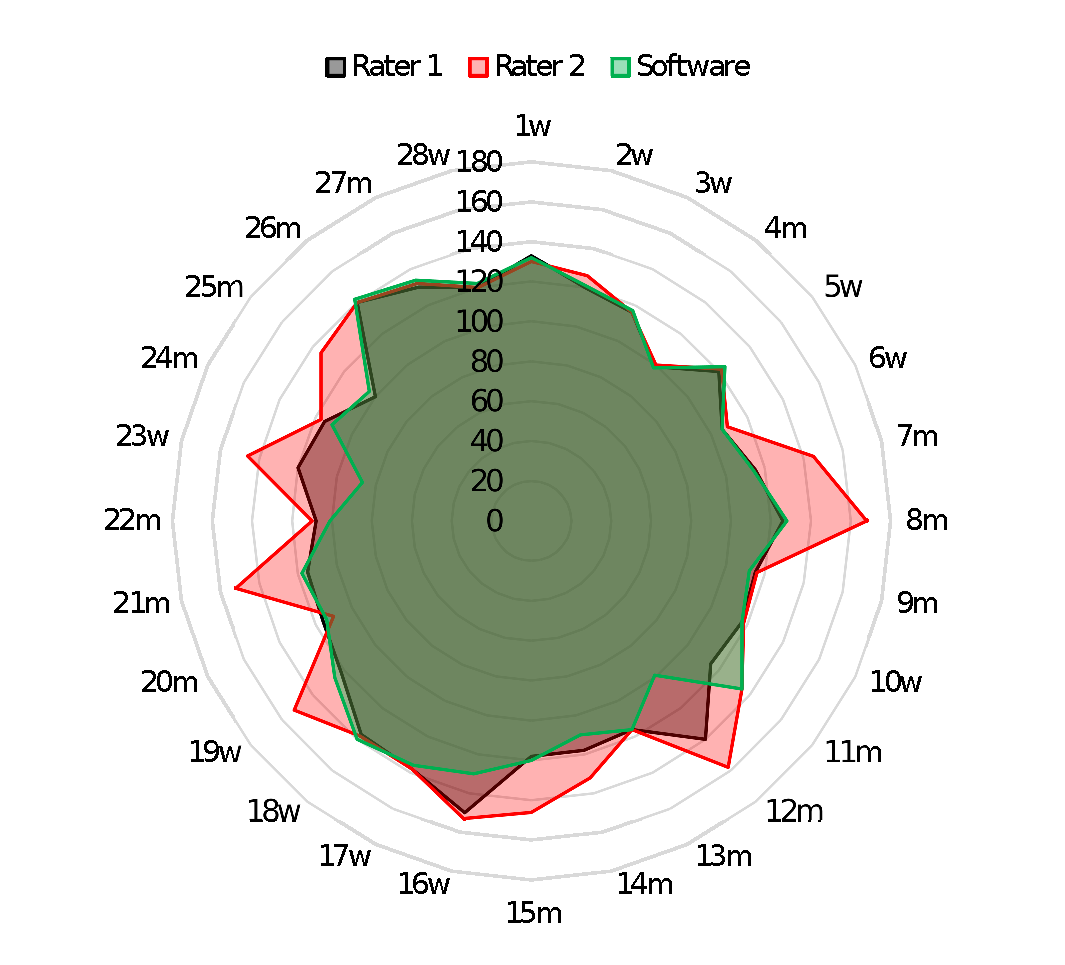
\includegraphics[scale=0.73]{Bilder/eqo2_net}
			\subcaption[Vergleich der VT1-Bestimmungen durch \acs{EQO2}]{Vergleich der VT1-Bestimmungen durch \acs{EQO2} zwischen Ratern und Software}
			\label{subpic:pic2}
	\end{subfigure}
\caption[Netzdiagramme zur Darstellung der Differenzen für VT1]{Zwei Netzdiagramme zur Darstellung der Differenzen zwischen Ratern und Software bei Bestimmung der VT1}
\label{pic:pic22}
\end{figure}
%
\begin{figure}[H]
	\centering
	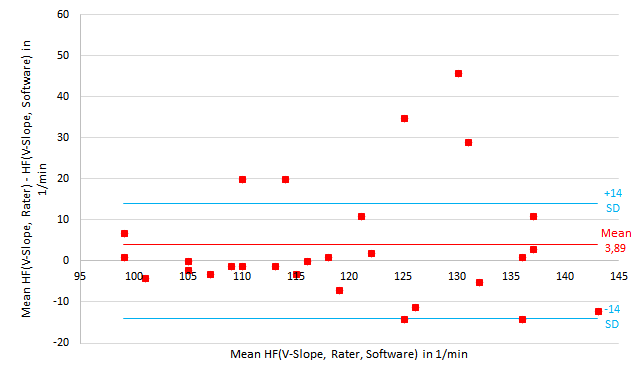
\includegraphics[scale=0.7]{Bilder/mean_vslope}
	\caption[Punktdiagramm mit Differenzen für V-Slope]{Punktdiagramm zur Darstellung der Differenzen zwischen den Mittelwerten für VT1 durch V-Slope von Ratern und Software mit Trendlinie und Standardabweichung}
	\label{pic:pic23}
\end{figure}
%
\begin{figure}[H]
	\centering
	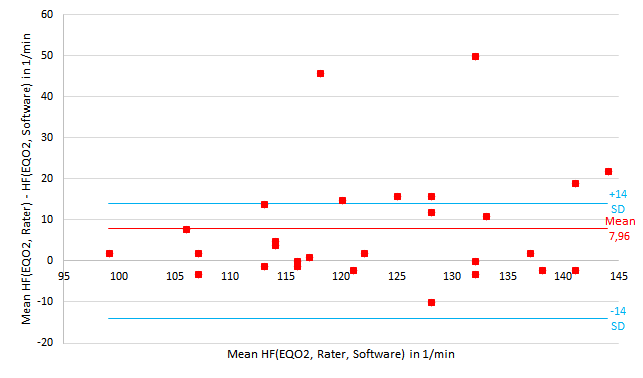
\includegraphics[scale=0.7]{Bilder/mean_eqo2}
	\caption[Punktdiagramm mit Differenzen für \acs{EQO2}]{Punktdiagramm zur Darstellung der Differenzen zwischen den Mittelwerten für VT1 durch \acs{EQO2} von Ratern und Software mit Trendlinie und Standardabweichung}
	\label{pic:pic24}
\end{figure}

Um die Schwellen zu vergleichen, wurden zusätzlich für jede Methode Punktdiagramme erstellt. In Abb. \ref{pic:pic23} ist ein solches für die V-Slope-Methode abgebildet. Die Y-Achse wird durch die Differenz aus der durchschnittlichen Rater-\acs{HF} und der Software-\acs{HF} im V-Slope in \si{\per\minute} definiert. Auf der X-Achse liegt der Durchschnitt aller drei einzelnen \acs{HF}, die für einen Probanden ermittelt wurden. Das Diagramm enthält 28 Messpunkte. Aus den Differenzen zwischen Ratern und Software wurde ein Gesamtdurchschnitt berechnet. Dieser ist im Diagramm als rote Linie sichtbar. Die VT1, die von Ratern und Software mittels V-Slope bestimmt wurden, unterscheiden sich durchschnittlich um \SI{3.89}{\per\minute}. Die \ac{SD} beträgt $\pm$14 \si{\per\minute}.\\
Abb. \ref{pic:pic24} zeigt das Diagramm für \acs{EQO2} mit den Differenzen zwischen Ratern und Software. Beim \acs{EQO2} beträgt diese im Mittel \SI{7,98}{\per\minute} bei einer \acs{SD} von ebenfalls $\pm$14 \si{\per\minute}.
\clearpage

\subsection{Ergebnisse für VT2}

\begin{table}[H]
	\begin{center}
		\caption{Ergebnisse für die \acs{HF} in \si{\per\minute} bei VT2}
		\medskip
		\begin{tabulary}{\textwidth}{L@{\hspace{3em}} C C C C C C C}
			\toprule
			& \multicolumn{2}{c}{\textbf{Rater 1}} & \multicolumn{2}{c}{\textbf{Rater 2}} & \multicolumn{3}{c}{\textbf{Software}} \\
			\midrule
			ID & \acs{EQCO2} & \acs{VE}/\acs{VCO2} & \acs{EQCO2} & \acs{VE}/\acs{VCO2} & \acs{EQCO2} & \acs{VE}/\acs{VCO2} & RQ=1 \\
			\midrule
			\midrule
			1w & 163 & 162 & 160 & 163 & 162 & 162 & 166 \\
			2w & 161 & 159 & 161 & 173 & 161 & 177 & 155 \\
			3w & 143 & 145 & 142 & 145 & 155 & 143 & / \\
			4m & 143 & 145 & 140 & 140 & 144 & 144 & / \\
			5w & 158 & 158 & 160 & 171 & 172 & 182 & 177 \\
			6w & 130 & 130 & 158 & 159 & 159 & 159 & 154 \\
			7m & 150 & 150 & 150 & 162 & 151 & 161 & 166 \\
			8m & 163 & 163 & 180 & 170 & 169 & 180 & 192 \\
			9m & 160 & 160 & 160 & 161 & 160 & 128 & 173 \\
			10w & 161 & 161 & 162 & 162 & 164 & 164 & 152 \\
			11m & 149 & 160 & 160 & 164 & 162 & 162 & 172 \\
			12m & 165 & 168 & 168 & 169 & 159 & 159 & / \\
			13m & 150 & 149 & 151 & 150 & 160 & 150 & / \\
			14m & 158 & 162 & 166 & 164 & 165 & 165 & 171 \\
			15m & 186 & 185 & 187 & 187 & 188 & 187 & / \\
			16w & 170 & 170 & 169 & 169 & 171 & 185 & 181 \\
			17w & 160 & 159 & 159 & 178 & 172 & 187 & 155 \\
			18w & 170 & 172 & 168 & 169 & 170 & 170 & 180 \\
			19w & 158 & 159 & 156 & 158 & 157 & 168 & 156 \\
			20m & 162 & 163 & 169 & 169 & 168 & 168 & 189 \\
			21m & 150 & 155 & 152 & 182 & 163 & 183 & / \\
			22m & 130 & 140 & 151 & 152 & 141 & 141 & / \\
			23w & 145 & 143 & 149 & 145 & 158 & 146 & / \\
			24m & 160 & 159 & 160 & 159 & 160 & 170 & 113 \\
			25m & 137 & 137 & 152 & 153 & 144 & 153 & / \\
			26m & 158 & 158 & 157 & 158 & 157 & 157 & 168 \\
			27m & 158 & 158 & 175 & 178 & 159 & 188 & 191 \\
			28w & 212 & 213 & 208 & 210 & 213 & 213 & 209 \\
			\bottomrule
		\end{tabulary}
		\label{tab:tabelle6}
	\end{center}
\end{table}

In Tab. \ref{tab:tabelle6} sind die \acs{HF} eingetragen, an denen Rater und Software die VT2 bestimmt haben. In dieser Tabelle wurde die Software-Spalte zusätzlich mit der Referenzmethode RQ = 1 ergänzt. Bei 9 von 28 Testmessungen konnte mit dieser Methode keine VT2 bestimmt werden, da die betroffenen Probanden dauerhaft einen RQ < 1 besaßen.

\begin{figure}[H]
	\centering
	\begin{subfigure}[c]{0.45\textwidth}
		\centering
		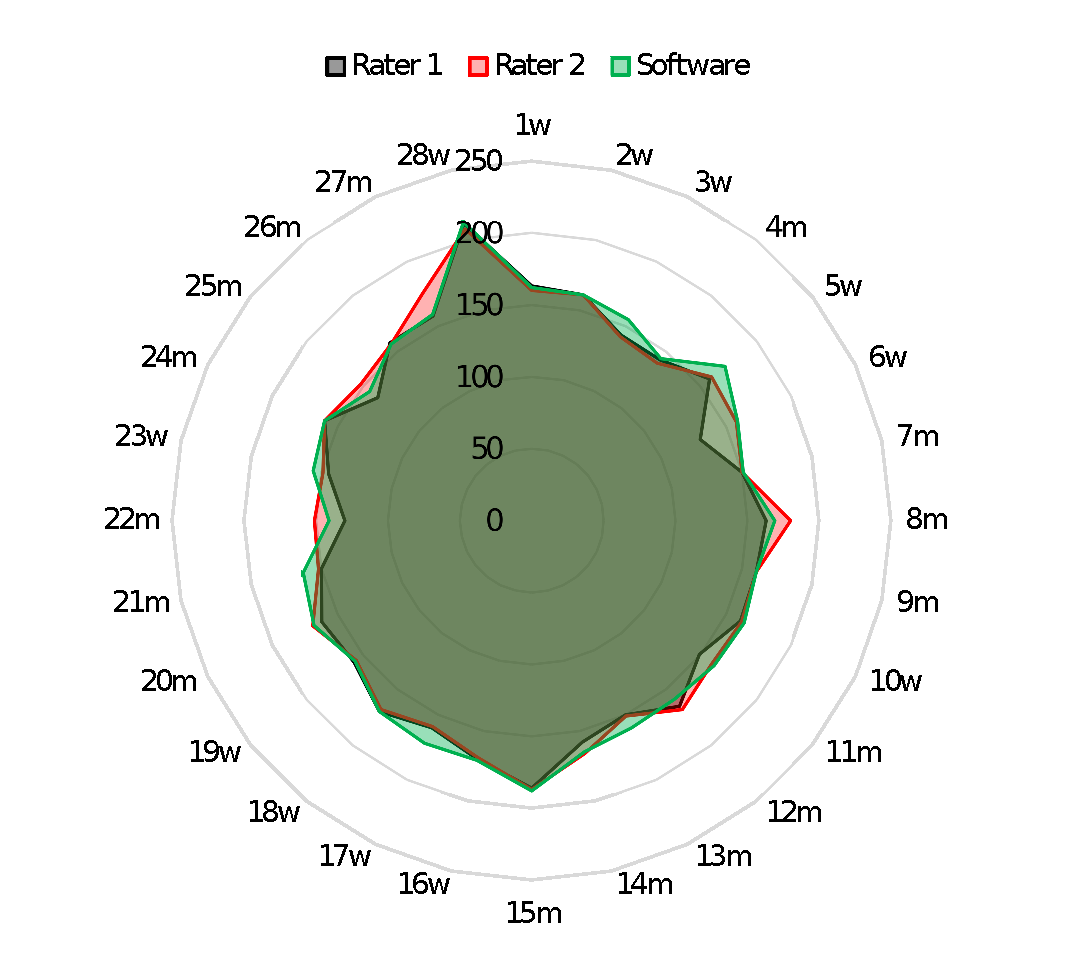
\includegraphics[scale=0.73]{Bilder/eqco2_net}
		\subcaption[Vergleich der VT2-Bestimmungen durch \acs{EQCO2}]{Vergleich der VT2-Bestimmungen durch \acs{EQCO2} zwischen Ratern und Software}
		\label{subpic:pic3}
	\end{subfigure}%
	\hfil
	\begin{subfigure}[c]{0.45\textwidth}
		\centering
		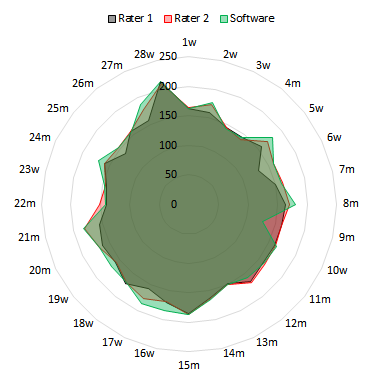
\includegraphics[scale=0.73]{Bilder/ve_vco2_net}
		\subcaption[Vergleich der VT2-Bestimmungen durch \acs{VE}/\acs{VCO2}]{Vergleich der VT2-Bestimmungen durch \acs{VE}/\acs{VCO2} zwischen Ratern und Software}
		\label{subpic:pic4}
	\end{subfigure}
	\caption[Netzdiagramme zur Darstellung der Differenzen für VT2]{Zwei Netzdiagramme zur Darstellung der Differenzen zwischen Ratern und Software bei Bestimmung der VT2}
	\label{pic:pic25}
\end{figure}

Abb. \ref{pic:pic25} zeigt die Netzdiagramme für die VT2-Ergebnisse durch \acs{EQCO2} und \acs{VE}/\acs{VCO2}. Diese sind bis \SI{250}{\per\minute} skaliert, da der höchste bestimmte Wert bei \SI{213}{\per\minute} liegt (siehe Tab. \ref{tab:tabelle6}).

\begin{figure}[H]
	\centering
	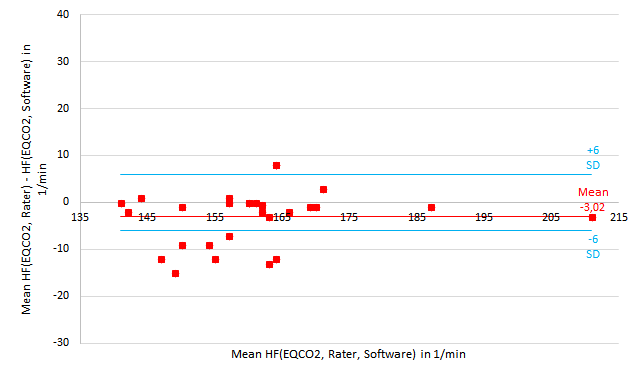
\includegraphics[scale=0.7]{Bilder/mean_eqco2}
	\caption[Punktdiagramm mit Differenzen für \acs{EQCO2}]{Punktdiagramm zur Darstellung der Differenzen zwischen den Mittelwerten für VT2 durch \acs{EQCO2} von Ratern und Software mit Trendlinie und Standardabweichung}
	\label{pic:pic26}
\end{figure}
\clearpage
In Abb. \ref{pic:pic26} ist das Diagramm für \acs{EQCO2} dargestellt. Die durchschnittliche Differenz für VT2, basierend auf \acs{EQCO2}, beträgt \SI{-3,02}{\per\minute}, während die \acs{SD} bei $\pm$6 \si{\per\minute} liegt.

\begin{figure}[H]
	\centering
	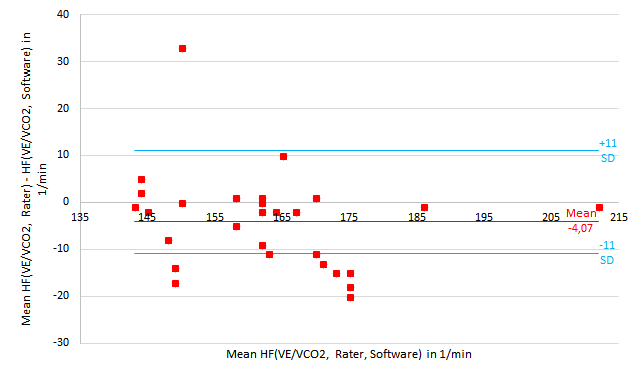
\includegraphics[scale=0.7]{Bilder/mean_vevco2}
	\caption[Punktdiagramm mit Differenzen für \acs{VE}/\acs{VCO2}]{Punktdiagramm zur Darstellung der Differenzen zwischen den Mittelwerten für VT2 durch \acs{VE}/\acs{VCO2} von Ratern und Software mit Trendlinie und Standardabweichung}
	\label{pic:pic27}
\end{figure}

Abb. \ref{pic:pic27} zeigt die Verteilung der Ergebnisse für \acs{VE}/\acs{VCO2}. Hier differieren Rater und Software um durchschnittlich \SI{-4,07}{\per\minute} bei einer \acs{SD} von $\pm$11 \si{\per\minute}.